\documentclass[12pt,a4paper]{article}
\usepackage[UTF8]{ctex}     %先引入ctex
\usepackage[utf8]{inputenc} %再引入inputenc
\usepackage[colorlinks,linkcolor=blue]{hyperref}
\usepackage{graphicx}
% \usepackage{lazylatex}
% \tcbuselibrary{documentation}
\usepackage{amsmath}
\usepackage{amssymb}
\usepackage{bookmark}
\usepackage{enumerate}
\usepackage{geometry}
\usepackage{tikz}
\usepackage{forest}
\usepackage{float}
\usepackage{multicol}
\usepackage{gbt7714}
\usepackage{array}
\usepackage{booktabs}
\usetikzlibrary{automata,positioning}

\graphicspath{{img/}}
% 边距
\geometry{left=2.0cm,right=2.0cm,top=1.0cm,bottom=3.0cm}
% 大题
\newenvironment{problems}{\begin{list}{}{\renewcommand{\makelabel}[1]{\textbf{##1}\hfil}}}{\end{list}}
% 小题
\newenvironment{steps}{\begin{list}{}{\renewcommand{\makelabel}[1]{##1)\hfil}}}{\end{list}}
% 答
\providecommand{\ans}{\textbf{答}:~}
% 解
\providecommand{\sol}{\textbf{解}.~}

\begin{document}
\title{\normalsize \underline{编译原理(A)}\\\LARGE第 5 次作业}
\author{Log Creative }
\date{\today}
\maketitle

\begin{problems}
    \item[1] 将下列正则表达式转换成DFA:
    \begin{steps}
        \item[a] $(a|b)^*$
        
        \sol 先转换为 NFA,

        \usetikzlibrary{graphs,rdf}
\tikzset{
dfa/.style = { semithick, > = To [sep] },
nfa/.style = { semithick, > = To [sep] },
state/.style = { circle, draw, minimum size = 1cm },
final/.style = { double },
initial/.style = { draw = red }, % to keep things simple
transition/.style = { edge label = {$#1$} }
}
\begin{tikzpicture}[nfa]
	\graph [math nodes, grow right = 1.5cm]{
		start ->
		0 [state,initial] -> [transition = {a,b}, loop below]
		0 -> [transition=a]
		1 [state] -> [transition = {a,b}, loop below]
		1 -> [transition=a]
		2[state] -> [transition = {a,b}, loop below]
		2 -> [transition=b]
		3[state, final];
		2 -> [transition=\epsilon,out=130,in=50]
		0;
	};
\end{tikzpicture}


        \begin{multicols}{2}
            DFA 转换表如下:
        
        \begin{tabular}{cc|cc}
            \hline
            NFA 状态 & DFA 状态 & $a$ & $b$ \\
            \hline
            \{0,1,2,3,7\} & $A$ & $B$ & $C$ \\
            \{1,2,3,4,6,7\} & $B$ & $B$ & $C$ \\
            \{1,2,3,5,6,7\} & $C$ & $B$ & $C$ \\
            \hline
        \end{tabular}

        最终 DFA 如右图所示。

        \usetikzlibrary {automata,positioning}
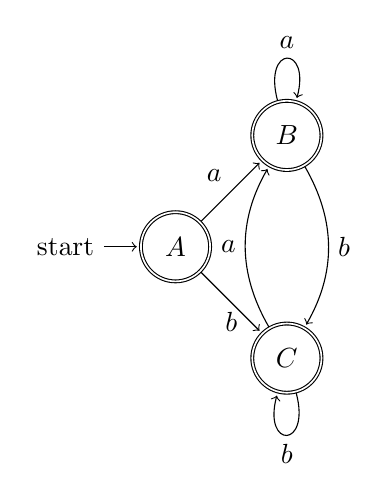
\begin{tikzpicture}[shorten >=1pt,node distance=2cm,on grid,auto]
	\node[initial,accepting,state] (A) {$A$};
	\node[accepting,state, above right of=A] (B) {$B$};
	\node[accepting,state, below right of=A] (C) {$C$};
	\path (A) edge[->] node {$a$} (B)
		(A) edge[->,below] node {$b$} (C)
		(B) edge[->,loop above] node {$a$} (B)
		(B) edge[->,bend left] node {$b$} (C)
		(C) edge[->,bend left] node {$a$} (B)
		(C) edge[->,loop below] node {$b$} (C);
\end{tikzpicture}


        \end{multicols}

        \item[b] $(a^*|b^*)^*$
        
        \sol 

        先转换为 NFA,

        \usetikzlibrary {automata,positioning}
\begin{tikzpicture}[shorten >=1pt,node distance=2cm,on grid,auto]
	\node[initial,state] (0) {0};
	\node[state,right of=0] (1) {1};
	\node[state,above right of=1] (2) {2};
    \node[state,below right of=1] (3) {3};
    \node[state,right of=2] (4) {4};
    \node[state,right of=4] (5) {5};
    \node[state,right of=5] (6) {6};
    \node[state,right of=3] (7) {7};
    \node[state,right of=7] (8) {8};
    \node[state,right of=8] (9) {9};
    \node[state,below right of=6] (10) {10};
    \node[accepting,state,right of=10] (11) {11};
    \path (0) edge[->] node {$\epsilon$} (1)
        (1) edge[->] node {$\epsilon$} (2)
        (1) edge[->] node {$\epsilon$} (3)
        (2) edge[->] node {$\epsilon$} (4)
        (3) edge[->] node {$\epsilon$} (7)
        (4) edge[->] node {$a$} (5)
        (7) edge[->] node {$b$} (8)
        (5) edge[->] node {$\epsilon$} (6)
        (8) edge[->] node {$\epsilon$} (9)
        (6) edge[->] node {$\epsilon$} (10)
        (9) edge[->] node {$\epsilon$} (10)
        (10) edge[->] node {$\epsilon$} (11)
        (0) edge[->,out=-90,in=-90] node {$\epsilon$} (11)
        (10) edge[->,out=90,in=90,above] node {$\epsilon$} (1)
        (2) edge[->,out=30,in=150] node {$\epsilon$} (6)
        (3) edge[->,out=-30,in=-150] node {$\epsilon$} (9)
        (5) edge[->,out=-90,in=-90,above] node {$\epsilon$} (4)
        (8) edge[->,out=90,in=90,below] node {$\epsilon$} (7);
	
\end{tikzpicture}


        \begin{multicols}{2}
            DFA 转换表如下:
        
        \begin{tabular}{cc|cc}
            \hline
            NFA 状态 & DFA 状态 & $a$ & $b$ \\
            \hline
            \{0,1,2,3,4,6,7,9,10,11\} & $A$ & $B$ & $C$ \\
            \{1,2,3,4,5,6,7,9,10,11\} & $B$ & $B$ & $C$ \\
            \{1,2,3,4,6,7,8,9,10,11\} & $C$ & $B$ & $C$ \\
            \hline
        \end{tabular}

        最终 DFA 如右图所示。

        \usetikzlibrary {automata,positioning}
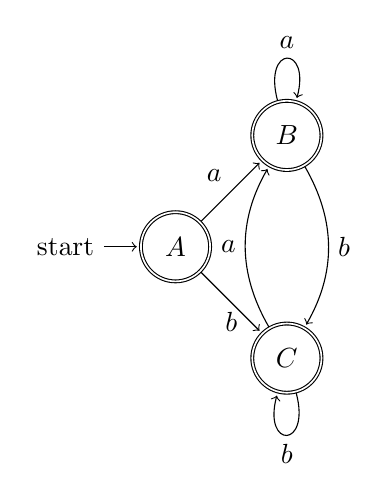
\begin{tikzpicture}[shorten >=1pt,node distance=2cm,on grid,auto]
	\node[initial,accepting,state] (A) {$A$};
	\node[accepting,state, above right of=A] (B) {$B$};
	\node[accepting,state, below right of=A] (C) {$C$};
	\path (A) edge[->] node {$a$} (B)
		(A) edge[->,below] node {$b$} (C)
		(B) edge[->,loop above] node {$a$} (B)
		(B) edge[->,bend left] node {$b$} (C)
		(C) edge[->,bend left] node {$a$} (B)
		(C) edge[->,loop below] node {$b$} (C);
\end{tikzpicture}


        \end{multicols}

        \item[c] $((\epsilon|a)b^*)^*$ 
        
        \sol 先转换为 NFA,

        \usetikzlibrary{graphs,rdf}
\tikzset{
dfa/.style = { semithick, > = To [sep] },
nfa/.style = { semithick, > = To [sep] },
state/.style = { circle, draw, minimum size = 1cm },
final/.style = { double },
initial/.style = { draw = red }, % to keep things simple
transition/.style = { edge label = {$#1$} }
}
\begin{tikzpicture}[nfa]
	\graph [math nodes, grow right = 1.5cm]{
		start -> 
		0[state,initial] ->[transition=\epsilon]
		1[state] ->[transition=\epsilon]
		2[state] ->[transition=\epsilon]
		3[state] -> [transition=a] 4[state] ->[transition=\epsilon]
		5[state] -> [transition=\epsilon]
		6[state] -> [transition=b] 7[state] ->[transition=\epsilon]
		8[state] ->[transition=\epsilon] 9[final,state];
		1 -> [transition=\epsilon,bend left] 4;
		5 -> [transition=\epsilon,bend left] 8;
		7 -> [transition=\epsilon,bend left] 6;
		8 -> [transition=\epsilon,bend left] 1;
		0 -> [transition=\epsilon,bend left] 9;
	};
\end{tikzpicture}


        \begin{multicols}{2}
            DFA 转换表如下:
        
        \begin{tabular}{cc|cc}
            \hline
            NFA 状态 & DFA 状态 & $a$ & $b$ \\
            \hline
            \{0,1,2,3,4,5,6,8,9\} & $A$ & $B$ & $C$ \\
            \{1,2,3,4,5,6,8,9\} & $B$ & $B$ & $C$ \\
            \{1,2,3,4,5,6,7,8,9\} & $C$ & $B$ & $C$ \\
            \hline
        \end{tabular}

        最终 DFA 如右图所示。

        \usetikzlibrary {automata,positioning}
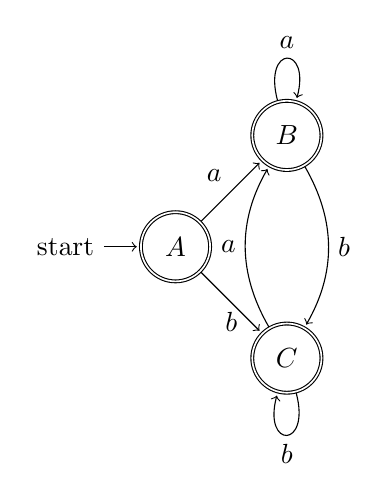
\begin{tikzpicture}[shorten >=1pt,node distance=2cm,on grid,auto]
	\node[initial,accepting,state] (A) {$A$};
	\node[accepting,state, above right of=A] (B) {$B$};
	\node[accepting,state, below right of=A] (C) {$C$};
	\path (A) edge[->] node {$a$} (B)
		(A) edge[->,below] node {$b$} (C)
		(B) edge[->,loop above] node {$a$} (B)
		(B) edge[->,bend left] node {$b$} (C)
		(C) edge[->,bend left] node {$a$} (B)
		(C) edge[->,loop below] node {$b$} (C);
\end{tikzpicture}


        \end{multicols}


    \end{steps} 
    \item[2] 对于深度学习编译器来说,表达一个深度神经网络的基本语言是什么?如果让你设计一种语言,并构造一种词法分析器,你会怎么做?你也可以替换成任何一种感兴趣的语言,如数据库查找SQL等。
    
    \ans 目前,大部分深度学习编译器表达深度神经网络的基本语言是 Python,由于 Python 较慢的速度也造成了一定的性能瓶颈。\cite{Li2021} 

    % 对于弱类型语言,比如 JavaScript,编译时才会对类型进行定义,词法也就需要在编译时根据上下文确定。而对于强类型语言,比如 TypeScript,词法在编译时就可以确定,这种词法分析器上下文无关。
    % 我会尽可能少的构造 DFA 的状态数目,使用 Lex 程序生成词法分析器。尽可能构造一种能用正则表达式识别的语言,减少编译器的构造难度。

    建立对于 \{\LaTeXe{} 命令\} -- \{\TeX{} 命令\} 子集的词法分析器(lexer)。这些命令用于 \textsf{AutoBeamer} 识别文档分块。

\textbf{词法单元}

\textsf{AutoBeamer} 主要识别两种基本的词法单元,正则描述如表 \ref{tab:basic-unit} 所示:
\begin{itemize}
    \item 命令(比如:\verb"\title{Slide Title}",命令参数是可选的)
    \item 英文词(比如:\verb"beamer")
    \item 其他语言的单字(比如:幻,灯,片)
\end{itemize}

\begin{table}[h]
    \centering
    \caption{\textsf{AutoBeamer} 所识别的基本词法单元}
    \label{tab:basic-unit}
    \begin{tabular}{>{\bfseries}c|cl}
        \toprule
        词法单元 & 非正式描述 & 正则描述\\
        \midrule
        command & 命令  & \verb"\\\w+(\[.*\]|\{.*\})*" \\
        word   & 词  & \verb"\w+" \\
        character & 字 & \verb"[^(\\|\w|\s)]" \\
        \bottomrule
    \end{tabular}
\end{table}

此外,对于命令语法单元,\textsf{AutoBeamer} 需要进行扩展识别,其相关正则描述如表 \ref{tab:extend-unit} 所示:
\begin{itemize}
    \item 环境开始(比如:\verb"\begin{document}")
    \item 环境结束(比如:\verb"\end{document}")
    \item 文档类(比如: \verb"\documentclass{article}")
\end{itemize}

\begin{table}[h]
    \centering
    \caption{\textsf{AutoBeamer} 所识别的命令扩展词法单元}
    \label{tab:extend-unit}
    \begin{tabular}{>{\bfseries}c|cl}
        \toprule
        词法单元 & 非正式描述 & 正则描述\\
        \midrule
        begin   & 环境开始  & \verb"\\begin{\w+}" \\
        end     & 环境结束  & \verb"\\end{\w+}" \\
        class   & 文档类    & \verb"\\documentclass(\[\w*\])?{\w+}" \\
        \bottomrule
    \end{tabular}
\end{table}

\textbf{构建 DFA}

确定的有穷自动机(Determinstic Finite Automata, DFA) 是构建词法分析器的重要依据。

基本的词法单元需要先识别命令,再识别词/字,其 DFA 如图 \ref{fig:basic-dfa} 所示。注意,输入的文件应该是已经可以通过 \LaTeX{} 编译的普通文档(不会出现 Error 异常,能输出 PDF 文档),所以 \verb"\" 后面应该就是字母,否则会报错。

\begin{figure}[h]
    \centering
    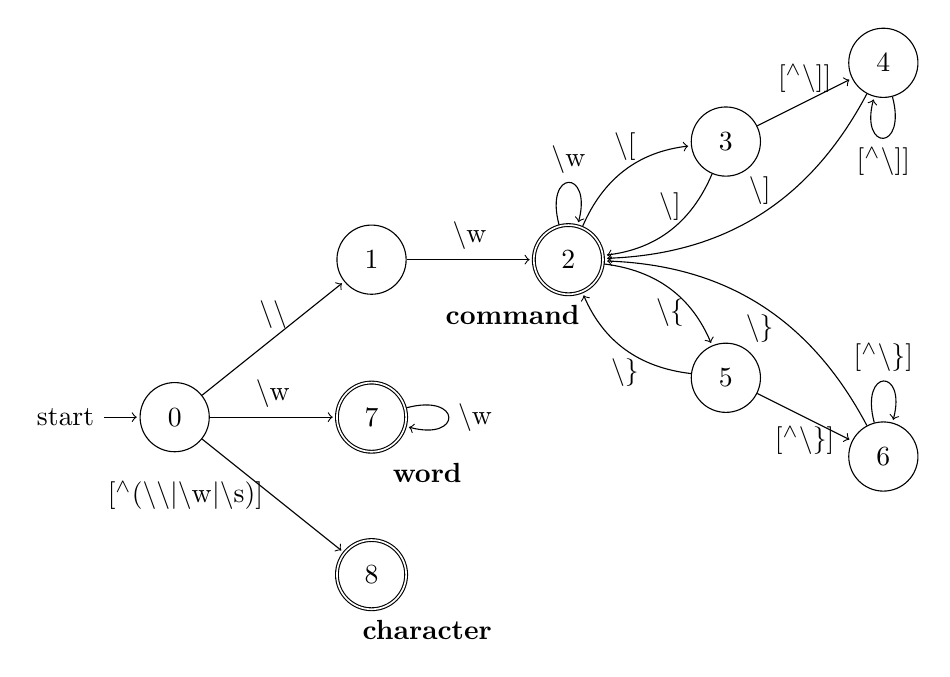
\begin{tikzpicture}[shorten >=1pt]
        \node[initial,state] (v1) at (-2,1) {0};
        \node[state] (v2) at (0.5,3) {1};
        \draw  (v1) edge[->] node[above] {$\backslash\backslash$} (v2);
        \node[accepting,state] (v4) at (3,3) {2};
        \draw  (v2) edge[->] node[above] {$\backslash$w} (v4);
        \draw (v4) edge[loop above] node {$\backslash$w} (v4);
        \node[state] (v5) at (5,4.5) {3};
        \draw  (v4) edge[->,bend left] node[above] {$\backslash$[} (v5);
        \node[state] (v6) at (7,5.5) {4};
        \draw  (v5) edge[->] node[above] {[$^\land\backslash$]]} (v6);
        
        \draw  (v6) edge[loop below] node {[$^\land\backslash$]]} (v6);
        \draw  (v5) edge[->,bend left] node[above] {$\backslash$]} (v4);
        \draw  (v6) edge[->,bend left] node[above] {$\backslash$]} (v4);
        \node[state] (v7) at (5,1.5) {5};
        \draw  (v4) edge[->,bend left] node[below] {$\backslash$\{} (v7);
        \draw  (v7) edge[->,bend left] node[below] {$\backslash$\}} (v4);
        \node[state] (v8) at (7,0.5) {6};
        \draw  (v7) edge[->] node[below] {[$^\land\backslash$\}]} (v8);
        \draw  (v8) edge[->,bend right] node[below] {$\backslash$\}} (v4);
        \draw  (v8) edge[loop above] node[above] {[$^\land\backslash$\}]}  (v8);
        
        \node[accepting,state] (v3) at (0.5,1) {7};
        \draw  (v1) edge[->] node[above] {$\backslash$w} (v3);
        \draw  (v3) edge[loop right] node {$\backslash$w} (v3);
        \node[accepting,state] (v9) at (0.5,-1) {8};
        \draw  (v1) edge[->] node[left] {[$\rm ^\land(\backslash\backslash|\backslash w|\backslash s)$]} (v9);
        
        \node [below left of=v4,font=\bfseries] {command};
        \node [below right of=v3,font=\bfseries] {word};
        \node [below right of=v9,font=\bfseries] {character};
    \end{tikzpicture}
    \caption{基本词法单元的 DFA}
    \label{fig:basic-dfa}
\end{figure}


对于命令扩展词法单元而言,需要有其已经是命令的先决条件,其 DFA 如图 \ref{fig:extend-dfa} 所示。仍然是在文档是编译正确的前提下进行的,如果没有匹配到扩展命令,将仍然作为 \textbf{command} 词法单元。

\begin{figure}[h]
    \centering
    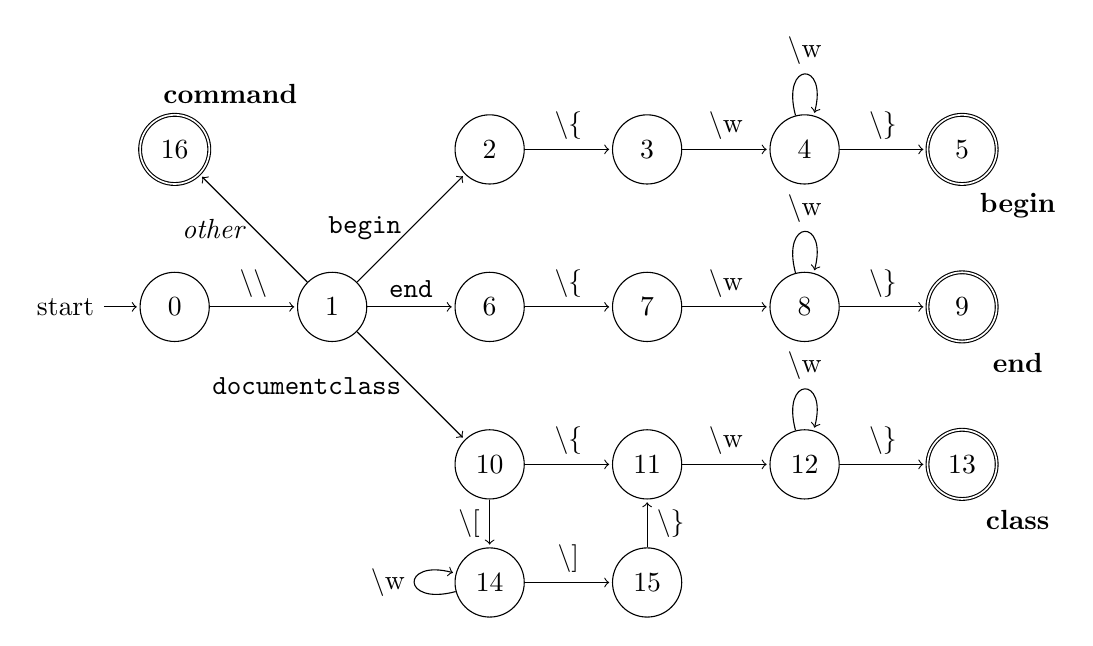
\begin{tikzpicture}[shorten >=1pt]
        \node[initial,state] (v1) at (0,0) {0};
        \node[state] (v2) at (2,0) {1};
        \draw[->]  (v1) edge node [above] {$\backslash\backslash$} (v2);
        \node[state] (v3) at (4,2) {2};
        
        \node[state] (v4) at (6,2) {3};
        \node[state] (v5) at (8,2) {4};
        \node[accepting,state] (v6) at (10,2) {5};
        \draw  (v2) edge[->] node[left,font=\ttfamily] {begin} (v3);
        \draw  (v3) edge[->] node[above] {$\backslash$\{} (v4);
        \draw  (v4) edge[->] node[above] {$\backslash$w} (v5);
        \draw  (v5) edge[loop above] node {$\backslash$w} (v5);
        \draw  (v5) edge[->] node[above] {$\backslash$\}} (v6);
        
        \node[state] (v7) at (4,0) {6};
        \node[state] (v8) at (6,0) {7};
        \node[state] (v9) at (8,0) {8};
        \node[accepting,state] (v10) at (10,0) {9};
        \draw  (v2) edge [->] node[above,font=\ttfamily] {end} (v7);
        \draw  (v7) edge [->] node[above] {$\backslash$\{} (v8);
        \draw  (v8) edge [->] node[above] {$\backslash$w}  (v9);
        \draw  (v9) edge [->] node[above] {$\backslash$\}}  (v10);
        \draw  (v9) edge[loop above]  node {$\backslash$w} (v9);
        \node[state] (v11) at (4,-2) {10};
        \node[state] (v12) at (6,-2) {11};
        \node[state] (v15) at (8,-2) {12};
        \node[accepting,state] (v16) at (10,-2) {13};
        \node[state] (v13) at (4,-3.5) {14};
        \node[state] (v14) at (6,-3.5) {15};
        \draw  (v2) edge[->] node[left,font=\ttfamily] {documentclass}(v11);
        \draw  (v11) edge[->] node[above] {$\backslash$\{}(v12);
        \draw  (v11) edge[->] node[left] {$\backslash$[}(v13);
        \draw  (v13) edge[->] node[above] {$\backslash$]}(v14);
        \draw  (v14) edge[->] node[right] {$\backslash$\}}(v12);
        \draw  (v12) edge[->] node[above] {$\backslash$w}(v15);
        \draw  (v15) edge[->] node[above] {$\backslash$\}}(v16);
        \draw  (v13) edge[->,loop left] node[left] {$\backslash$w} (v13);
        \draw  (v15) edge[->,loop above] node[above] {$\backslash$w}  (v15);
        \node[accepting,state] (v17) at (0,2) {16};
        \draw  (v2) edge[->] node[font=\itshape,left] {other} (v17);
        
        \node[below right of=v6,font=\bfseries] {begin};
        \node[below right of=v10,font=\bfseries] {end};
        \node[below right of=v16,font=\bfseries] {class};
        \node[above right of=v17,font=\bfseries] {command};
    \end{tikzpicture}
    \caption{命令扩展词法单元的 DFA}
    \label{fig:extend-dfa}
\end{figure}

DFA 构建完毕后,就可以编写对应的词法分析器了,后续的代码进展请进入:

\href{https://github.com/LogCreative/AutoBeamer/tree/main/src/lexer}{https://github.com/LogCreative/AutoBeamer/tree/main/src/lexer}。

\end{problems}

\bibliography{hw05.bib}

\end{document}
